\chapter{アプリケーション層}



インターネットプロトコルスイートそのもののしめくくりとして、、TCP/IPを通信手段として利用するアプリケーション層について説明をします。

ネットワークアプリケーションを、インターネットプロトコルイートにおけるアプリケーション層として見直していくことからはじめましょう。

\section{アプリケーション層とはなにか}

アプリケーション層とは、おおまかに説明すれば、ホスト上で動作するプロセスである。そのプロセスが、他のプロセスとの通信に、TCP/IPのトランスポート層のサービスを使用すれば、そのプロセスはTCP/IPにおけるアプリケーション層となる。
他のプロセスへの通信に、トランスポート層を使用するのであれば、通信相手のプロセスは自分自身を含むどのホストで動作していてもかまわない。

たとえば、メールサーバのアプリケーションは、他のホストのメールサーバやメールクライアントのソフトと、トランスポート層の機能を使って通信する。そのため、TCP/IPでいうところのアプリケーション層である。また、データベースなど、一見ネットワークと関係なさそうなアプリケーションでも、データベースを利用する他のアプリケーションとの通信に、TCP/IPを用いていれば、アプリケーション層のアプリケーションである。
アプリケーションのプロトコルは、その目的によって規定されている。

一般に、トランスポート層としてTCPを用いるアプリケーションは、人間が可読な、短いテキストを交換しあう、テキスト指向のプロトコルとなることが多い。また、UDPを用いるアプリケーションは、メッセージを短くするために、バイナリデータをやりとりするプロトコルとなることが多い。

\subsection{プロセス間通信}
TCP/IPにおけるアプリケーション層を考えるに当たって、まず、プロセス間通信というものを考えよう。それにあたって、ここではプロセスとアプリケーションという言葉を、ホストの上で動くプログラム、という同じ意味で使うことにする。

そもそも、プロセス間通信は何のために行うのだろうか。

例として、ユーザがアクセスして何か登録をするアプリケーションを考えてみよう。まず、登録のインタフェイス、内部にデータとしてため込むロジックをひとつのアプリケーションとして作ったとする。
この場合は、ユーザはそのアプリケーションが動いているホストを直接操作できる場所に行く必要がある。また、あるホストの上で動くアプリケーションに登録されたデータを、他のアプリケーションから再利用することもできない。
ではまず、ユーザインタフェイスを分離して、インタフェイスとデータを登録するアプリケーションの間は、プロセス間通信を行うことにする。

それによって、ユーザは、アプリケーションが動作するホストとプロセス間通信が可能な端末を使えば、どこからでもこのアプリケーションを利用することができる。

次に、アプリケーション側で、ユーザ側のインタフェイスと通信するフロントエンドと、データを保存管理するデータベースを別のアプリケーションにしよう。必要なデータの交換は、このアプリケーションの間のプロセス間通信で行うものとする。

これによって、ユーザインタフェイスと通信するアプリケーションを複数のホストで動作させて冗長性を確保することができる。また、データを管理する部分も、それ専用のアプリケーションとしいう、シンプルな形でで実装できる。

このように、アプリケーションを、シンプルな機能のアプリケーションがお互いに通信しながら実行される形にする。それによって、それぞれのアプリケーションを汎用勝つ単機能にすることができる。

実はこれは、一般的なWebサービスサーバの環境である。クライアントであるWebブラウザ、フロントエンドであるWebサーバ、データを管理するデータベースのそれぞれがプロセス間通信を行うことで、ひとつのサービスが実現されている。



\subsection{アプリケーション層ではないプロセス}
TCP/IPのトランスポート層をサービスとして利用し、他のプロセスと通信を行うプロセスがアプリケーション層である、そう説明した。これは、あるプロセスがプロセス間通信を行っていても、その通信手段にTCP/IPのトランスポート層を使用していなければ、TCP/IPのアプリケーション層ではないということである。

UNIX系のOSでは、プロセス間通信にはいくつか手段がある。パイプを使用する場合は当然アプリケーション層ではない。また、プロセス間通信にソケットを使用する場合でも、UNIXドメインソケットを使用する場合は、これもまたTCP/IPアプリケーション層でなはない。

くり返すが、TCP/IPのトランスポート層のサービスを使用するのが、TCP/IPのアプリケーション層である。だが、プロセス間通信の手段にTCP/IPを使っていないだけであることに注意をした。


\section{ポート番号の選択}
あるホストの上では、複数のアプリケーションが動作している。たとえば、同じホストの上でメールサーバとWebサーバが稼働しているような場合が考えられるだろう。このとき、アプリケーション層のひとつ下のレイヤであるトランスポート層は、それぞれのアプリケーションをどのように区別するかを、アプリケーション層の視点で振り返ってみよう。

アプリケーションは、ポート番号と呼ばれる、0から65535までの、16bit長のユニークな番号を、トランスポート層とのインタフェイスに割り当てる。その番号を発信元、受信先に更に割り当てる音で、それぞれを区別する。
たとえば、トランスポート層とのインタフェイスに2048というポート番号を割り当てたアプリケーションがあった場合、トランスポート層は、2048番宛ての通信は全て、そのアプリケーションに送る。

そのため、プロセス間通信の相手を指定する場合は、ホストの場所の情報と別に、そのホストにおけるどのポート番号を宛先とするかを指定しなければならない。

また、同じポート番号を、複数のアプリケーションが使うことはできない。例えば、あるホストの上で、80番のポートを、Webサーバとメールサーバに割り当てたとしよう。このとき、ネットワーク経由で、メールクライアントからも、Webブラウザからも、80番ポート宛てに通信が来る。
だが、トランスポート層は、これがメールサーバ宛ての通信なのか、Webサーバ宛ての通信なのかを決定できない。トランスポート層以下のレイヤーは、ペイロードを解釈しない。
逆に、同じアプリケーションのプロセスが、それぞれ異なるポート番号を割り当てられた状態で動作しているという状態は許容される。たとえば、80番で通信するWebサーバと、91番で通信するWebサーバが、同じホストの上で動作していてもかまわない。

ここまでで、アプリケーションにではなく、トランスポート層とのインタフェイスに番号を割り当てる、という表現をした。これは、ひとつのアプリケーションが、複数のポート番号を持つ場合があるためだ。
たとえば、FTPは20番と21番という二つのポートを使用する。

ポート番号を表記するときは、スラッシュをつけた後に、使用するトランスポート層のプロトコルを併記することが多い。例えば、SMTPで使用する25番ポートに、TCPを用いて通信することを表す際は、25/TCPというように記述する。同様に、UDPを用いるプロトコルであるDNSであれば、53/UDPというように記述する。

\subsection{ウェルノウンポート}
アプリケーションが通信を行うときは、通信相手のアプリケ=ションがどれかを特定するための情報として、ポート番号が必要となる。そのため、よく知られたアプリケーション層のプロトコルは、あらかじめポート番号が予約されている。そのポート番号を、ウェルノウンポート(Well-Known-Port)と読んでいる。

ウエルノウンポートは0-1023番の範囲であり、IANA(Internet Assigned Numbers Authority)という団体が管理している。

あるプロトコルを使用するアプリケーションでは、トランスポート層のインタフェイスに割り当てるポート番号が、予約されているということだ。
たとえば、メールのプロトコルであるSMTPは25番ポートを、ウェルノウンポートとして割り当てられている。そのため、メールを転送する場合は、どこのホストが宛先でも、送信先ホストの25番ポートを宛先として指定すればSMTPの通信ができることを期待されている。


\subsection{登録済ポート (Registerd port)}

ポート番号1024-49151番の範囲を、登録済ポート(Registerd Port)と呼び、どのアプリケーション層のプロトコルに、どのポートを割り当てるか、という指針をIANAが公開している。

\subsection{動的割り当て/プライベートポート (Dynamic and/or Private port)}

クライアントアプリケーションが通信に使用するポートとしては、49152-65535番の範囲の利用が推奨されている。この範囲を、動的割り当て/プライベートポート(Dynamic and/or Private port)と読んでいる。

例えば、Webブラウザのように、ユーザによって任意のタイミングで起動、終了するアプリケーションの場合は、ポート番号は空いているところから動的に割り当てる方が効率がよい。

\subsection{ポート番号の割り当て状況を見る}

ポート番号の割り当て状況を見るには、/etc/servicesファイルの中身を見ればよい。このファイルには、主要なサービスに割り当てられたポート番号の一覧が記載されている。\footnote{/etc/servicesでは、ウェルノウンポートと登録済みポートについて、くアプリケーション層のプロトコル名と、対応するポート番号が記載されている。これは、そのアプリケーションプロトコルを使用するアプリケーションで、そのポートを利用するように、という意味である。}

以下、そのファイルの一部を抜粋してみよう。プロトコルと、対応するポート番号がひとつの行に記載されている。同一プロトコル名で複数記述卯があるのは、同じポート番号でTCPを使う場合、UDPを使う場合のそれぞれについて予約がされているからである。

\begin{verbatim}
ssh              22/sctp   #Secure Shell Login
ssh              22/tcp    #Secure Shell Login
ssh              22/udp    #Secure Shell Login
telnet           23/tcp
telnet           23/udp
#                24/tcp    any private mail system
#                24/udp    any private mail system
smtp             25/tcp    mail         #Simple Mail Transfer
smtp             25/udp    mail         #Simple Mail Transfer
\end{verbatim}

\section{アプリケーション層のプロトコル}

アプリケーション層のプロトコルとは、何らかの通信手段を利用できることを前提に、プロセスとプロセスが情報を交換するための手順である。その通信手段とは、プロトコルが求めるものを満たすのであれば、TCP/IPのトランスポート層でなくても構わない。

このような書き方をした理由は、TCP/IP以前に考案され、その時代から使われているプロトコルも多いためだ。たとえば、SMTPやtelnetは、TCP/IP成立前から使用されてきたレガシーなプロトコルである。

アプリケーション層のプロトコルは、、テキスト指向のものバイナリ符号のものに分けることができる。

テキスト指向というのは、エンドツーエンドで送信されるメッセージもしくはコマンドが、可読なテキストであるプロトコルを指す。バイナリデータのストリームを流すこともできるが、その際はBase64やQuoted Printableによるエンコードを用いて、テキストデータにエンコードして、テキストデータとして通している。

元々はTCP/IP成立以前に使われていたプロトコルの形態であった。だが、その可読性から、今でも使用され、開発されているプロトコルである。

テキスト指向のプロトコルは、可読であるため、コマンドの組立や戻ってくるメッセージの判別を簡単に行うことができる。だが、アプリケーションではコマンドやもどってきたメッセージを解釈して次の動作を決定するパーサが必要となる。そのため、テキスト指向のプロトコルの戻りメッセージでは、文字列の先頭に3桁の数字列をつけ、その部分だけみればサーバからの応答が分かるようになっている場合が多い。この3桁の数字をリザルトコードという。

バイナリ符号のプロトコルは、ビット列やワードの値を解釈することで、コマンドやパラメータをやり取りするもの、アプリケーション層が送受信するデータに、そのプロトコル独自のヘッダがつくものなど、テキスト指向でないプロトコルを、バイナリ符号であるとする。

\subsection{トランスポート層の選択}

ここまで、テキスト指向とバイナリ符号のそれぞれのプロトコルが、TCPとUDPのどちらを使うか、という点に関しては論議をしなかった。
テキスト指向のプロトコルはTCPを利用することが多い。これは、多くの場合、コマンドによってアプリケーションが状態遷移するプロトコルであるため、コマンドや結果のメッセージの送受信に確実性が求められるためである。同様の理由で、バイナリ符号のプロトコルでも、TCPを利用するものがある。

一方、UDPは、バイナリ符号型のプロトコルが多い。これは、データ部分にアプリケーション層の制御情報をヘッダとしてのせたり、データロガーの一方的なデータ転送に用いられたり、TCPのオーバヘッドが許容できない状況で送信されるデータであるなど、UDPを用いるアプリケーション事に起因する理由である。UDPデータグラムひとつに収まる長さで(UDPなので、複数データグラムの到着順保証はない)、一部データグラムが欠落、つまりコマンドやメッセージそのものが失われても、それをアプリケーション側で補償するプロトコルを構築すれば、テキスト指向のプロトコルにUDPを用いることも可能である。

ひとつ気をを付ける点があるとすれば、アプリケーション層とトランスポート層の間に依存関係がない、というのは、プロトコルがトランスポート層に依存していないという意味である。アプリケーションソフトウェアの実装は、必ずトランスポート層に依存する。その問題は、本省の後に改めて説明をしたい。


\subsection*{いもうとコラム TLS}
TCP/IPにおいて通信を暗号化し、プロセス通信の相手の正当性を確認するプロトコルとして、TLS(Transport Layer Security)というものがあります。以前はSSL(Secure Socket Layer)と呼んでいたものを改良したものであるため、バージョンを意識しなくて言い場面では、SSLという名前で呼ばれることも多いものです。

TLSについては専門書が何冊もありますので、ここでは、TLSがTCP/IPにおいてどこの層に属するかを考えてみることにします。

このプロトコルの実装は、OSI参照モデルに当てはめた場合は例や5のセッション層に当てはめられることが多いです。また、TLSを使用するアプリケーションを実装するときは、TLSのライブラリ経由でソケットを使用します。そうすることで、トランスポート層以下は、暗号化したデータが送信され、アプリケーションが受け取るデータは、TLSが復号化したものとなります。

では、TLSはTCP/IPのどのレイヤーにいるプロトルなのでしょうか。実のところ、TCP/IPにおける実装としては、TLSは、アプリケーション層のプロトコルになります。

その理由は、トランスポート層、それもTCPのコネクション指向を利用して、エンドと暗号化した通信を行うという実装に寄ります。特に、トランスポート層が通信の順序を担保することを前提としてます。

そのため、通信順が担保される、コネクション指向のトランスポート層プロトコルであれば、理論上、TCP出ないプロトコルでもTLSは通信を行うことができます。

トランスポート層から見れば、TLSはサービスを行うべきアプリケーション層となることに注意してください。



アプリケーション層のプロトコルは、おおまかに

\subsection{テキスト指向のプロトコル}

テキスト指向のプロトコルの例として、電子メールに用いられるシンプルメール転送プロトコル(SMTP Simple Male Transfer Protocol)を取り上げる。SMTPは、1980年にMail Transfer Protocolの名前でRFC772として提案された後、1982年にRFC821として、最初のSMTPが提案され、インターネットにおける弟子メールの標準プロトコルとなった。その後、各種の拡張を経て現在では2008年10月提案のRFC5321が最新版となっている。

現在は、TCPのポート番号25番をサーバの待ち受けとして使用することが多い。\footnote{プロバイダによっては自社メールサーバ意外の25番ポートへのアクセスをブロックするOPB25を行っていることがある。企業のメールサーバなど、社員が任意の接続元からそのメールサーバを利用したい場合は、送信時認証とセットにしてSubmission 587/TCPで待ち受ける設定を行う。}

SMTPのサーバアプリケーションは、サーバでありクライアントである。クライアントから接続され、転送するメール受信する過程はサーバの動作であり、そのメールが他のメールサーバに転送すべきものであれば、クライアントとして宛先となるメールサーバに接続する。そのため、SMTPを解説する際は、コネクションをアクティブオープンする方をクライアント、パッシブオープンする方をサーバとして捉え、説明することが多い。3)

SMTPで、メールサーバに接続して、サーバにメールを渡すまでの手順を追っていくことにしよう。SMTPは、1行1コマンドのプロトコルで、クライアントからのコマンドに対し、サーバは1行以上のリザルトを返す。

\begin{table}[hbtp] \caption{Simple Male Transfer Protocol(SMTP)} \label{smtp}
\begin{center}
{\footnotesize
	\begin{tabularx}{13cm}{llXX} \toprule
	時間 & クライアント側コマンド & サーバ側リザルト & 概要 \\ \midrule
	1 & HELO host.hoge.tld & - & クライアント側ホスト名を通知してセッション初期化 現在、ほとんどの実装ではIPの発信元フィールドから拾う \\ \hline
	2 &  -  & 250 host.fqdn.tld & HELOコマンド了承 \\ \hline
	3 & MAIL FROM: from@hoge.tld & -  & 発信元メールアドレスを通知 SMTPのコマンドで通知されるのがエンベローブ(封筒)情報である \\ \hline
	4 & -  & 250 Ok &	MAILコマンド了承 \\ \hline
	5 & RCPT TO: mailto@fuga.tld & - & 宛先メールアドレスを通知 SMTPのコマンドで通知されるエンベローブ(封筒)情報 最近の実装では、同報する宛先の数繰り返すことが可能なものも多い \\ \hline
	6 &  -  & 250 Ok & RCPTコマンド了承 \\ \hline
	7 & DATA & -  & メールの転送を開始したい \\ \hline
	9 & \shortstack{ From: from@hoge.tld \\ To: mailto@fuga.tld \\ Subject: tes \\   \\   \\ test mai \\ . } &  - & メールデータ入力  ここで入力されるFrom:やTo:などの情報は、メールのヘッダとなる \\ \hline
	10 & -  & 250 Ok: queued as C71681EBAE0 & メールデータ受付を記載のキューIDで受け付け \\ \hline
	11 & QUIT & - & クライアントよりセッション終了を通知 \\ \hline
	12 & -  & 221 Bye & サービス切断 \\ \bottomrule
	\end{tabularx}
}
\end{center}
\end{table}


ここで、クライアント側からのメール送信元ならびに宛先を、SMTPコマンドとして送信し、DATAコマンド以降のメールデータの送信でも、データの一部として送信している。これはどちらかでいいのではないか、と思わないだろうか。実際には、メール本文でのFrom:やTo:は省略でき、その場合はMAILコマンドやRCPTコマンドの引数が用いられる。

だが、このように、計算機やネットワークの資源が乏しかった時代に成立したにもかかわらず、冗長な使用となっているのには理由がある。それは、SMTP は、英文の手紙の書式を模しているためである。まず、英文の手紙の書式を考えてみよう。英文の手紙では、レターヘッドに発信元の情報、日付、宛先、件名が必ず記載される。その手紙が封筒(エンベローブ)に入れられ、配送に使われる宛先や発信元は封筒に記載される。

MAILコマンドやRCPTコマンドで送信される発信元、宛先の情報を、エンベローブ(封筒)情報という。エンベローブ情報は、サーバが宛先にメールを転送するために用いる情報である。そのため、MAILとRCPTは必須の情報で、メールデータ側で省略された場合のデフォルト値としても用いられる。

メールデータ側のFrom:やTo:などの情報は、メールヘッダという。メールヘッダは、前述の通り、英文の手紙の書式に由来する。では、FromやTo が、エンベローブ情報と異なった場合はどうなるだろうか? メールヘッダとエンベローブ情報が異なる場合、配信にはエンベローブ情報が使われる。このエンベローブ情報は、通常は受信したユーザは見ることができない。ユーザが見ることができるのは、メールヘッダの情報である。エンベローブ情報は、メールヘッダでFromやToが欠落している場合のみ、そのデフォルト値として使われる。これが何を意味するかというと、CCやBCCの宛先にメールを送信するときの動作である。CC(Carbon Copy)は、宛先でないが同報したことを開示してメールを送る先、BCC(Blind Carbon Copy)は、メールを同報したことを伏せてメールを送信する宛先である。どちらも、転写紙(Carbon)を敷いて同じ文面のメールを複数枚同時にタイプライタで作成していたことに由来する。

CCやBCCに記載された宛先は、ヘッダ情報のToにはない。だが、SMTPコマンドのRCPTで、クライアントからメールサーバに宛先として通知される。BCCの場合は、クライアントがBCC行の情報をメールヘッダから取り除いた上で、その宛先をRCPTコマンドでメールサーバに通知する。それによって、メールヘッダのTo に宛先がなくても、メールがCCやBCCに記載した宛先に到着する。


\subsection{バイナリ符号のプロトコルの例}

次は、バイナリ符号プロトコルの例として、トリビアルファイル転送プロトコル(TFTP Trivial FTP)を紹介しよう。TFTPは最低限のファイル転送を行うためのプロトコルである。用途として、ディスクレス機器に、システム立ち上げに必要なファイル転送を行うことを想定している。

その実装は実行バイナリがディスクレスの機器のEPROMに収まるサイズになることを最優先としている。そのため、ファイル転送以外のファイル操作、認証などの機構をもたない。また、プロトコルスタックもEPROMに収まるサイズにするため、TCPと比較したときにバイナリの小さいUDPを、トランスポート層として採用している。サーバの待ち受けポートは69/UDPが用いられる。

これまでも記載したとおり、トランスポート層としてTCPやそれ以外を用いてもかまわないが、TFTP本来の目的から外れるため、そのような実装例はない。TFTPは、現在ではネットワーク機器へのファームウエアのアップロードなどに使用されている。

\subsubsection{TFTPのパケットフォーマット}

TPTPメッセージは、5種類のオプコード(opcode)と、4種類のパケットフォーマットを持つ。TFTPメッセージは、トランスポート層にUDPを使用するので、UDPデータグラムのデータ部分として送出される。フォーマットが4種類しかないのは、送信要求と受信要求が、同一のパケットフォーマットを使用するからである。

TFTPメッセージは、先頭2オクテットがオプコードとなる。それ以降は、オプコードによって異なる。

\paragraph{RRQ/WRQパケット}

RRQ/WRQパケットは、読み書きするファイルのファイルネームと、転送モード名の文字列を通知する。ファイルネームとモードは、1オクテットの0で区切る。転送モード名は、8bitで改行コードにCRLFを用いるnetasciiと、無変換の8bitコードであるoctetである。\footnote{古いTFTPの規格では、もうひとつmailモードというものがあるが、RFC1350では、mailモードは廃止するので対応してはならないことになった}

TFTPには、読み書きするファイルのパスにchdirする機能はない。TFTPでアクセスするディレクトリは、ディスクレスクライアントの起動用ファイルの読み出しの場合は多くの場合決め打ち、それ以外の場合は、アプリケーション側でサポートすることになる。

\begin{figure}[htbp]
	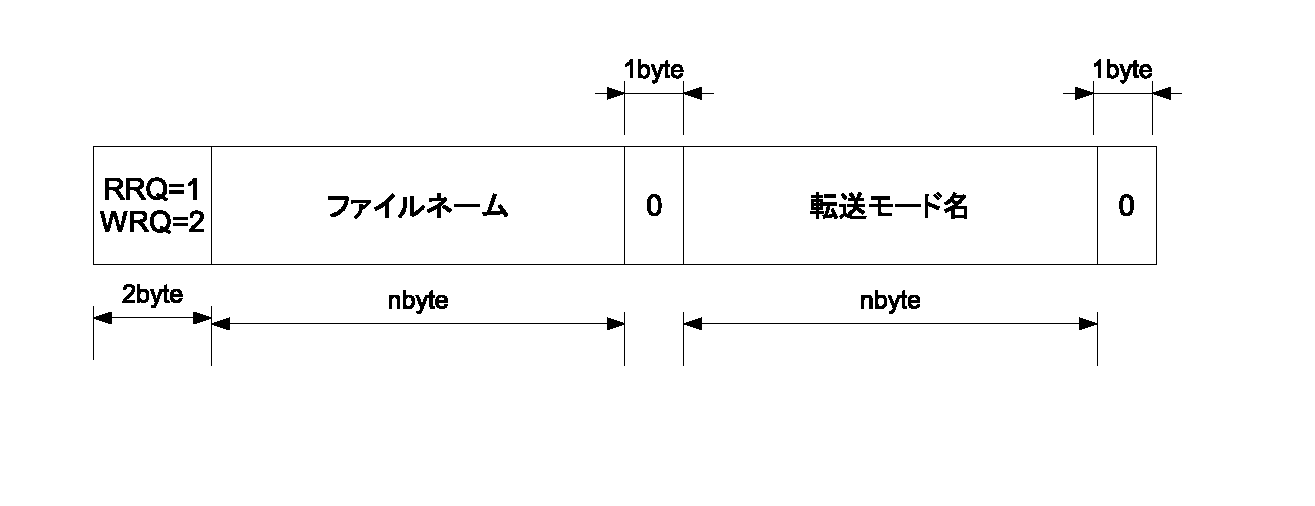
\includegraphics[width=12cm,clip]{draw/tftp_op1.eps}
	\caption{RRQ/WRQパケット}
	\label{fig:ftfp_op1}
\end{figure}


\paragraph{DATAパケット}

\begin{figure}[htbp]
	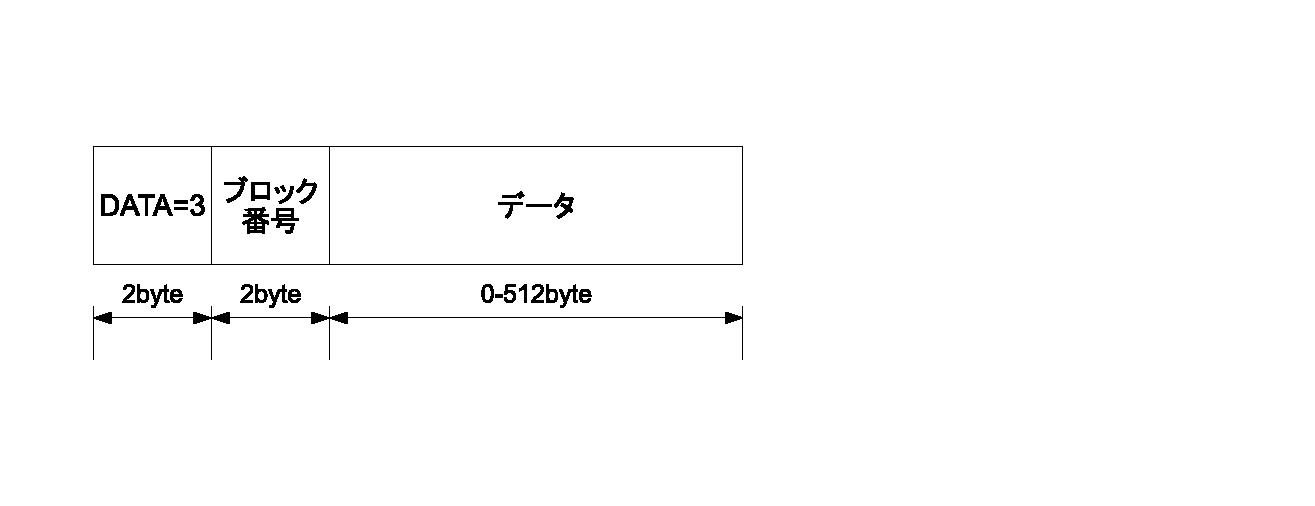
\includegraphics[width=7cm,clip]{draw/tftp_op2.eps}
	\caption{DATAパケット}
	\label{fig:ftfp_op2}
\end{figure}

DATAパケットは、パケットの順番を表す2バイトのブロック番号をもつ。データ部分のサイズが512オクテットであればそれはファイルの末尾ではない。 0から511オクテットであればデータはそのパケットで終了である。ブロック番号は1から開始される。

\paragraph{ACKパケット}

ACKパケットは、DATAパケットの到着を通知するのに用いる。ブロック番号は、到着を確認したデータパケットのブロック番号となる。 TCPのACKにおける確認応答番号でないことに注意してほしい。RRQ/WRQパケットにたいしてもACKを返すが、そのときはブロック番号0 を用いる。

\begin{figure}[htbp]
	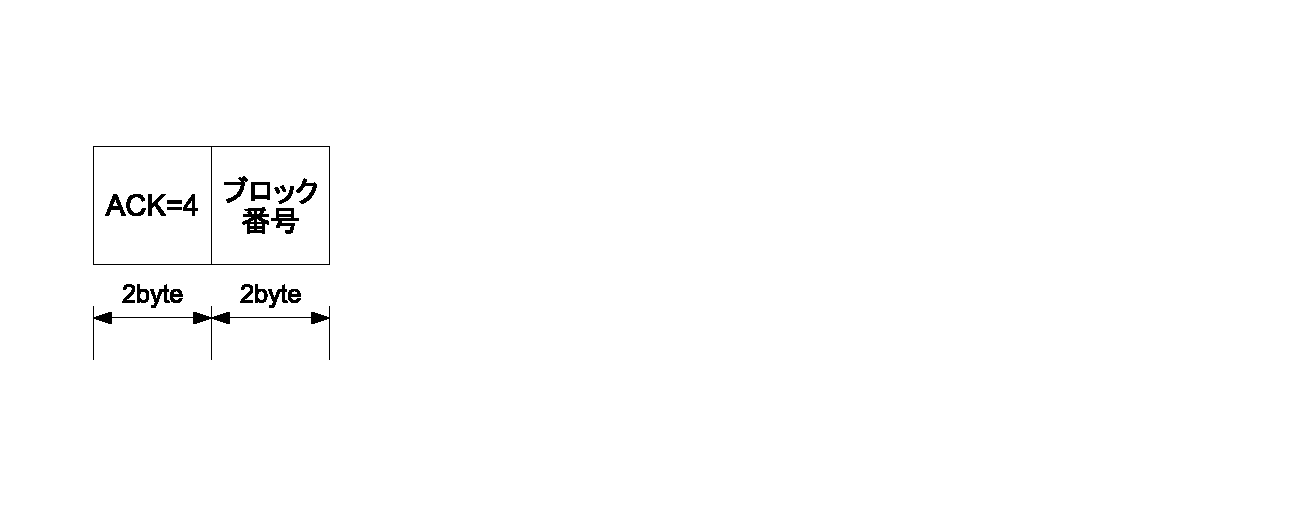
\includegraphics[width=12cm,clip]{draw/tftp_op3.eps}
	\caption{ACKパケット}
	\label{fig:ftfp_op3}
\end{figure}

\paragraph{ERRORパケット}

\begin{figure}[htbp]
	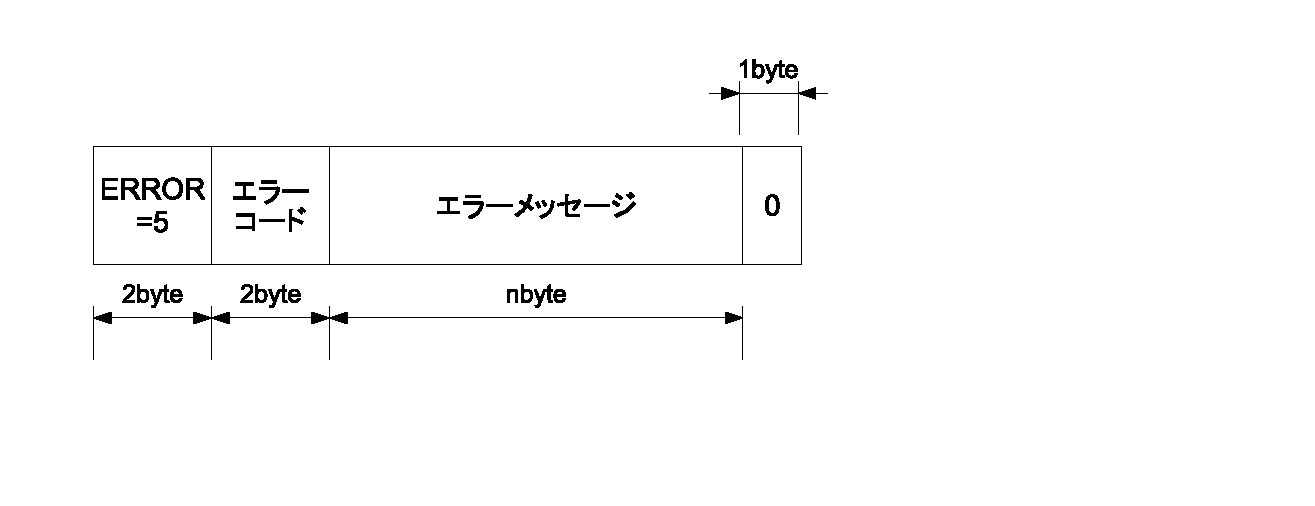
\includegraphics[width=12cm,clip]{draw/tftp_op4.eps}
	\caption{ERRORパケット}
	\label{fig:ftfp_op4}
\end{figure}


ERRORパケットは、エラーが発生した際に、他のパケットへの確認応答として送出される。ErrorCodeフィールドは0-7の8種類のエラーコードのうちどれかを指定する。メッセージフィールドは人間が確認するためのもので、netascii形式で可読な文字列を入れるべきである。


\subsubsection{TFTPの通信手順}

次に、TFTPの通信手順について説明しよう。TFTPでは、サーバとクライアントが、ごく簡単な制御情報を交換しながらデータをやりとりするプロトコルである。

なお、このTFTPには、魔法使いの弟子シンドロームというアルゴリズムバグがある。その内容と解決方法については付録に追記したので、そちらを参照していただきたい。

\paragraph{コネクション確立}

TFTPサーバは、69/UDPで待ち受ける。クライアントからRRQ/WRQパケットが送られてきたら、サーバはランダムで新しいポートを選択し、それをUDPデータグラムの発信元ポートに設定して、ACKパケットを送信する。RRQ/WRQパケットに対するACKパケットのブロック番号は0である。

それ以降の通信では、クライアントの使うポートと、サーバがRRQ/WRQパケットを受け取ってからランダムに決定したポートとの間で通信が行われる。それ以降は69/UDPは使用されない。

\paragraph{データ転送}

それ以降は、クライアントからWRQパケットでコネクションが開始された場合として説明しよう。サーバからのACKを受信したクライアントは、DATAパケットを送信する。そのブロック番号として、ACKについているブロック番号の、次の番号をもつブロックを送信する。クライアントは、送出したDATAパケットのブロック番号に対応したACKを受信するまで、次のブロックは送信しない。これは、ストップアンドウエイト(調歩式)と呼ばれるプロトコルである。

\paragraph{データのエラーチェック}

TFTPのデータのエラーチェックは、トランスポート層(UDP)で行われることが期待されている。エラーになった(チェックサム不一致の)UDPデータグラムに積まれていたパケットは、UDPで破棄される。

\paragraph{再送処理}

TFTPの再送処理は、送信側のみがタイマーを持ち、時間内にACKが戻らなければそのパケットを再送する。重複ACKを受信したときに、それに対応するブロック番号のデータを再送してはならない。

DATAを受信する側は、新しいDATAパケットが届くはずの状況でDATAパケットが届かないときに、ACKを再発行して「催促」する動作はしない。TFTP では、受信側はタイムアウト処理とそれに伴う再請求は行わない。

\paragraph{コネクション切断}

TFTPのコネクション切断は、512バイト未満のデータ部分もつ(つまり長さが516バイトより短い)DATAパケットを受信したときか、エラーが発生したときである。この場合は、ACKは送信されない。つまり、TCPのFIN-ACKに相当するシーケンスはない。



\section{ソケットとアプリケーションの実装}
これまでも説明したとおり、アプリケーション層のプロトコルとトランスポート層の間には、プロトコルにおける依存関係はない。だが、実装に関しては、依存関係が生ずる。

4.2BSDより、アプリケーションが別のプロセスと通信するための経路を抽象化したインタフェイスとして、socket(2)が導入された。本書では、ソケットとsocket(2)を便宜上同じ概念として扱うことにする。

そのアプリケーションがTCP/IPのアプリケーション層である場合は、ソケットを経由して、トランスポート層のサービスを利用するように実装する。

\subsection{ソケット}

ソケットは、プロセス間通信の経路を抽象化したものである。そのため、TCP/IP以外のネットワークプロトコルを使用できる実装もある。アプリケーションが、TCP/IPにおけるトランスポート層のサービスを使うという用途に限定されたインタフェイスではないことに注意をしたい。

また、同一ホストの上で動作するプロセス間の通信であれば、ネットワーク経由ではなく、UNIXドメインソケットという、、同一ホスト場のプロセス間の通信を使うこともできる。UNIXドメインソケットは、ネットワークを使用するソケットよりも使用するリソースが少なくてすむこと、また、副次的な利点として、同一ホスト以外のプロセスとは通信できないこと、という利点がある。

リアルタイム性が失われたり、ネットワークアクセス層に流れるビットが多くなってもかまわないなら、UDPを使用しているアプリケーション層のプロトコルに、TCPを使用することも可能である。逆に、経路の信頼性を引き替えにし、それによって生ずる不都合をアプリケーション層で吸収できるなら、本来TCPでやり取りしていたプロトコルに、UDPを利用することもできる。



\subsection{ソケットのアドレスファミリ}
ソケットでプロセス間通信の通信路を開くとき、インターネットプロトコル層のアドレスで通信相手を指定しなければならないことは前述の通りである。そして、もうひとうつ、インターネットプロトコルスイートを利用するためにソケットを使うなら、IPv4とIPv6のどちらで通信をするか、それを指定する必要がある。

通信相手がどのようなアドレス体系のアドレスで特定されるのかも、アプリケーションが指定しなければならない。このアドレス体系のことをアドレスファミリという。

インターネットプロトコル層を使うのであれば、IPv4ならAF\_INETを指定する。また、IPv6ならAF\_INET6を指定する。AF\_IENT6を指定した場合は、IPv4とIPv6のどちらからのアクセスも受け入れるソケットとなる。

\subsection{ネットワークバイトオーダと htonl()}

IPアドレスは、32ビット(4byte)を単位としたビット列としてネットワークコミュニケーション層に渡される。このときの送出順は、0ビット目(図\ref{fig:ipheader}の左側)から31ビット目(図\ref{fig:ipheader}の右側)にむけて「ビッグ・エンディアン」方向となる。これを、ネットワーク・バイトオーダという。

だが、x86系CPUなどは、24ビット~31ビット、16ビット~23ビット、8ビット~16ビット、0ビット~7ビットという、バイト単位で見たときにネットワークバイトオーダと逆順にメモリにコピーする仕様となっている。このような環境をリトル・エンディアンという。

そのため、プログラミングでIPアドレスを\verb+sockaddr_in+ 構造体にコピーする際に、\verb+htonl()+ という関数で、IPアドレスのビット列を、ネットワークバイトオーダで出力されるよう順番を入れ替えてから渡す。

一方、PowerPCやColdFireなど、ビッグエンディアンな環境では \verb+htonl()+ は不要なように思われる。だが、コードの移植性を考えて、常に\verb+htonl()+ を使用しておくようにする。\footnote{エンディアン変換の必要のない環境では\verb+htonl()+ は何もしないマクロとして定義されている。}

IPv6でもネットワークバイトオーダを考える必要がある。\verb+sockaddr_in6+ 構造体の\verb+in_addr6+には、ネットワークバイトオーダでアドレスを書き込む。これは、アドレスファミリAF\_INET6を指定したときは、IPv4とIPv6のどちらのアドレスも受け付ける。その互換性維持のためである。

\subsection{名前解決という問題}
TCP/IPのアプリケーション層としてアプリケーションを実装する場合には、トランスポート層以下を意識しなければならないという問題がある。具体的には、インターネットプロトコル層を意識しなければならない場面が生じる。これは、本来はトランスポート層以下のサービスを意識しなくてもよい、という、インターネットプロトコルスイートの概念からは反してしまう部分である。

プロセス間通信を行うときは、当然、アプリケーションのレベルでの「宛先」を意識する。概論で用いたたとえを用いれば、アプリメーション層が意識する宛先は、たとえば、「京都市役所」のようなシンボルの名前である。これは、プロセス間通信の相手の場所を表す名前、つまりURL(Unique Resource Location)という概念である。

この、場所を表す名前から、その場所をポイントする住所、つまりアドレスの変換する、もしくは住所からそこにあるものの名前の対応関係を調べることを、ネットワークの用語では、名前解決という。

今の知見で考えれば、URLであらわされる通信相手の居場所が京都市役所であれば、それを住所である京都市中京区寺町通り御池上ル本能寺前に変換するのは、おそらくインターネットプロトコル層の仕事であろう。
だが、ソケットの実装では、名前解決を行うのは、アプリケーションが行わなければならない。アプリケーションが、本来は触れなくていいはずのインターネットプロトコル層の情報である、IPアドレスをソケットに与えるという仕様になっている。これは歴史的な経緯から、現在のソケット実装でも変更されていない。

そのため、アプリケーションの実装において、IPv6への対応はアプリケーションでも行う必要があるという問題が残っている。TCP/IPの概念通り、アプリケーション層が実装においてもトランスポート層以外を意識しなくてもかまわないならば、そもそもアプリケーション層でのIPv6対応は行う必要がないものであった。

いささか余談ではあるが、IPv6への対応にはアプリケーションの対応も必要となるのは、このような理由があるためである。


\subsection*{いもうとコラム なぜ名前解決をアプリケーションが行うのか}
アプリケーションが名前解決を行わなければならない歴史的経緯とは何なのでしょうか。ソケットという概念が4.2BSDに実装された頃の時代背景も併せて考えてみることにしましょう。

まず考えられるのは、URLにおける場所の記述としては、ホスト名もIPアドレスも使用されるという観点です。アプリケーション層でプロセス間通信の相手のURLを記述するために、IPアドレスを使わない、名前だけで行う、というのは、現実問題として難しいです。実際の運用では、名前の付いていないホストはいくらでもあります。

そんな、アドレスはあっても名前を持っていないホストと通信するときは、アプリケーションもIPアドレスを使用せざるを得ません。トランスポート層の情報じゃないから、というわけにはいかないのです。

そうなると、インターネットプロトコル層で、トランスポート層から渡されたデータの中にあった宛先が、名前解決が必要な名前なのか、必要ないIPアドレスかを判断して、必要であれば名前解決を行う、という実装をするのが正しいのか、それを考えなければなりません。

コンピュータのリソース、特にネットワーク処理のコストが高かった時代には、データグラムの送信ごとにインターネットプロトコル層でその判定を行って名前解決をするよりも、アプリケーション側で最初に名前解決をして、プロセス間通信が完了するまではその結果を使い続けるという実装が選択されても不思議ではなかったでしょう。

もうひとつ、初期のインターネットにはDNSがなかったという点も覚えておく必要があります。当時から名前解決の概念はありましたが、初期はテキストファイルにホスト名とIPアドレスを1行一組で記述していました。そのテキストファイルを、新しいホストがインターネットに追加されるごとに更新して、FTPで配布していたわけです。

そのため。テキストファイルを読んで、名前解決を行うという実装は、インターネットプロトコル層には組み入れられなかった、むしろアプリケーションで行うべき都判断された、というのは想像に難くありません。

ちなみに、その、FTPで配布していたテキストファイルの名残が、/etc/hostsです。たいていの名前解決の実装で、このファイルの記述情報は最優先で参照されることになっています。


\subsection{トランスポート層の選択}
これまでも説明したとおり、アプリケーション層のプロトコルとトランスポート層の間には、依存性はない。

だが、TCP/IPのトランスポート層を利用する実装を行うのであれば、複数あるトランスポート層のプロトコルの何を使うのか、その選択をする必要がある。

TCPは、データの送信順の維持も含めて、確実な通信を提供する。これをコネクション指向という。そのかわり、確実な通信を成立させるためのコストが高く、リアルタイム性を求められる通信にはあまりむいていない。

一方のUDPは、処理が軽く、リアルタイム性を求められる、音声や動画の伝送にも剥いている。そのかわり、確実性はなく、データの送信順が意味を持つプロトコルの場合は、アプリケーション側でデータの到着順などを管理しなければならない。そのため、コネクションをつくらない、コネクションレス型と呼ばれる。


\subsection{アプリケーションサーバの実装}

では、トランスポート層においてTCPを使用するアプリケーションと、UDPを使用するアプリケーションの違いは何であろうか?

プロトコルで、サーバとクライアントが対話するものはTCP、対話しないものはUDP、という印象があるかもしれない。だが、TCPとUDPのどちらを使用するかは、UDPで間に合うか、TCPの信頼性が必要か、で決められることが多い。
サーバとクライアントが対話、つまり「プロセス間通信を繰り返して動作するSMTPやHTTPは、多くの場合TCPが用いられる。これは、対話はデータの到着順が意味を持つため、アプリケーションがデータの到着順を意識しなくてよいTCPが多く用いられる。

トランスポート層としてUDPを使用するアプリケーション層のプロトコルでは、アプリケーション層のプロトコルが、フロー制御などを受け持つことがある。これは、ストリーミングなど、データの再送よりも、データが送られてくることを優先したいアプリケーションにおいて採用される実装である。

また、SNMPやsyslogのように、不特定のリモートホストから送出されるデータを待つタイプのサービスも、UDPが使われることが多い。\footnote{sysぉgは、TCPを用いる置き換え実装が現れてきている。これは、TCPコネクションの維持にかかるコストが低くなったことと、UDPによるデータ取りこぼしをなくす、というような意図がある。}

\section{サーバの実装}
アプリケーション層であるアプリケーションの実装は、大きく分けて反復型と並行型の二種に分類できる。

反復型は、単一のプロセスが、ソケットから通信を受けると、それに対する処理をして結果を返す。これを繰り返すものである。反復型は、クライアントからの質問にサーバが回答すれば終了するプロトコルの実装で用いられる。この場合、応答に要する時間が短いこと、複数クライアントからの問い合わせがあってもそれをバッファに置いて逐次処理する場済む、という用件がある場合に採られる。

一方の並行型は、クライアントとサーバが、対話するプロトコルで使用されることが多い。対話するということは、通信の終了までの時間が予想できないということである。このときに他のクライアントから通信を求められた場合、反復型のプロセス処理では、待ち時間が判らない状況でクライアントを待たせることになる。

そこで、並行型は、クライアントからアクセスがあれば、プロセスをforkして、以降の通信は子プロセスが行う。親プロセスは、待ち受けと子プロセスの生成を担当する。それによって、複数クライアントからの同時問い合わせへの対応を可能とする。

反復型サーバはUDP、並行型サーバはTCPを用いることが多い。だが、TCPでも反復型の実装をされるプロトコルもあれば、UDPでも並行型の実装をされるプロトコルもある。そのため、一概に言うことはできない。

また、TCPとUDPの最大の違いである、コネクション指向かどうか、という点でも、アプリケーション実装における相違が生ずる。TCPを使用する場合は、 accept(2)によってコネクションが成立したら、以降はそのファイルデスクプリタからデータをrecv(2)し、send(2)すればよい。これは、コネクション確立によって、データがどこからきているか、データをどこに送るべきかが確定しているからである。一方UDPでは、コネクションレスであるため、受信時にどこから来たデータグラムかを確認し、応答が必要であれば、問い合わせを送ってきたところを宛先としてデータグラムを送信するようにしなければならない。

UDPを使用する場合は、アプリケーション層で受信したデータの送信元を確認し、どこに送信するかをデータグラム毎に設定する必要がある。そのため、アプリケーションの実装では、手間がかかるように思える。実際に、クライアントでUDPを使用するときは、connect(2)を、送信先のデフォルト値を決定するために使うことが多い。


\subsection{TCPの反復型サーバ}
次に、TCPを用いた反復型サーバの実装を見ることにしよう。先に説明したとおり、例は多くないが、TCPでも反復型サーバの実装が行われる場合がある。

{\scriptsize
\begin{verbatim}
// ソケットと待ち受けキューの準備
fd = socket(AF_INET,SOCK_STREAM,0);
bind(fd);  // ファイルデスクプリタに、待ち受けIPアドレスとポートで名前を付ける
listen(fd,BACKLOG);  // コネクション待ち受けキューをつくる。BACKLOGは待ち受けキュー長

while( 1 ){
    newfd = accept( fd );  // 待ち受けキューに何かはいるまでブロック 3way handshakeする。

    //
    // newfdと通信して何らかの処理をする
    //

    close(newfd);
}
\end{verbatim}
}

\subsection{UDPの反復型サーバ}
UDPは、反復型サーバとして実装されることが多い。これは、UDPが、確認応答が必要なく、比較的単純なメッセージのやりとりに使用されることが多いためである。

{\scriptsize
\begin{verbatim}
// ソケットと待ち受けキューの準備
fd = socket(AF_INET,SOCK_DGRAM,0);
bind(fd);  // ファイルデスクプリタに、待ち受けIPアドレスとポートで名前を付ける

while( 1 ){
    rcvfrom( fd , buf , buflen , flag , from , fromlen);  // recvfromはデータグラム到着までブロック
 
         //
        // bufに入っている受信データへの応答を作成
         //
 
        sendto( fd, msg , msglen , flag , to ,tolen );  // 通常toはfromと同じ(メッセージ送信元に返信する)
}
\end{verbatim}
}

\subsection{TCPの並行型サーバ}
TCPを用いるサーバは、並行型サーバとして実装されることが多い。これは、確実な通信を保証するTCPは、ホスト間の対話を行うサーバアプリケーションに使用されることが多いためである。

{\scriptsize
\begin{verbatim}
// ソケットと待ち受けキューの準備
fd = socket(AF_INET,SOCK_STREAM,0);
bind(fd);  // ファイルデスクプリタに、待ち受けIPアドレスとポートで名前を付ける
listen(fd,BACKLOG);  // コネクション待ち受けキューをつくる。BACKLOGは待ち受けキュー長

while( 1 ){
    newfd = accept( fd );  // 待ち受けキューに何かはいるまでブロック 3way handshakeする。
    if( 0 == fork() ){
        // 子プロセス
        close( fd );

       //
       // newfdと通信して何らかの処理をする
        //

        close(newfd);
       exit(EXIT_SUCCESS);
    } else {
        // 親プロセス
         close( newfd );
    }
}
\end{verbatim}
}


\subsection{スーパーデーモン}

最近では使われることが少なくなりつつあるが、アプリケーション層には、スーパーデーモンという特別なアプリケーションを経由する実装の方法がある。最後にその説明を行うことにしよう。

UNIX系のOSには、inetd\footnote{セキュリティを強化した置き換えアプリケーションに、xinetdなどがある。最近はxintedの方をデフォルトで使用する場合も多い}というデーモンがある。これは、TCP やUDPの指定されたポートで待ち受け、コネクションが確立、もしくはデータグラムが受信されれば、ポート毎に指定されたアプリケーションを起動するサーバアプリケーションである。だが、inetdは、ここまでで説明したような並行型の動作ではない。

inetdは、指定されたポートで通信を待ち受ける。そして、TCPのコネクションが成立、もしくはUDPデータグラムが受信されたら、指定されたアプリケーションを子プロセスとして起動する。通常の並行型アプリケーションでは、フォーク時にコピーされたファイルデスクプリタを使って、通信を含めた全処理を子プロセスに投げる。

だが、inetdは、子プロセス側の標準入出力を、inetdが待ち受けしたソケットにリダイレクトする。つまり、inetdで起動されるアプリケーションは、標準入出力にさえ対応していれば、ネットワーク対応のコードが不要となる。これは、実行バイナリがディスクにしめる容量も削減できるということでもある。また、標準入出力を使用するアプリケーションであれば、ネットワーク対応でなくてもinetd経由で、ネットワーク越しに利用することが可能となる。

このように、アプリケーション(デーモン)の管理をするアプリケーションであるため、inetdには、スーパーデーモンという別名がつけられている。
では、何のためにスーパーデーモンという形態の実装が行われたのであろうか。

昔は、メモリもHDDも容量単価がたかく、ホストに搭載できる容量の上限も小さかった。UNIX系のOSは仮想記憶をサポートしているとはいえ、クライアントからの接続を待っている時間の方が長いサーバアプリケーションを、複数常駐させるだけのリソースがなかった。そのため、スーパーデーモンが代表してTCPと UDPの各ポートでの待ち受けを行い、コネクションが確立、もしくはデータグラムが到着したら、実際の処理を担当するサーバアプリケーションを起動する、という方法が採られた。

スーパーデーモン経由でのサーバアプリケーションへのアクセスは、その起動待ち時間と、ソケットを標準入出力にリダイレクトする処理で、クライアントから見たレスポンスは低下する。また、近年の、ソケットを使用する実装のネットワーク対応アプリケーションをスーパーデーモン経由で利用しようとすれば、逆に、標準入出力の利用を意識したコードが必要となる。

そのため、コンピュータリソースのコストが下がった現在では、スーパーデーモンを使用せず、必要なデーモンを予め起動しておく運用が行われる。

だが、スーパーデーモンは、古くからあるアプリケーションのためにに残されている。たとえば、BSD標準のTFTPデーモンは、inetd(8)から起動される実装のまま、使用されている。

